\documentclass[a4paper,11pt]{article}%,twocolumn
\input{settings/packages}
%% page settings
\usepackage[top=10mm, bottom=15mm,left=10mm,right=10mm]{geometry}  
 % needed for page border settings
\parindent=0mm % for space of first line of new text block

\sloppy % for writing with hyphenless justification (tries to)
\hyphenation{} % use hyphenation of tolerance parametershttp://www.jr-x.de/publikationen/latex/tipps/zeilenumbruch.html
\hyphenpenalty=10000
\exhyphenpenalty=10000
\usepackage{fancyhdr} % needed for head and foot options
\input{settings/jupyter}

\begin{document}
	\begin{center}
	{\large \textbf{Assignment A04: Neural Networks}}\\
	Thalagala B.P.\hspace{0.5cm} 180631J 
\end{center}
\hrule


%    \begin{tcolorbox}[breakable, size=fbox, boxrule=1pt, pad at break*=1mm,colback=cellbackground, colframe=cellborder]
%\prompt{In}{incolor}{1}{\boxspacing}
%\begin{Verbatim}[commandchars=\\\{\}]
%\PY{k}{def} \PY{n+nf}{sigmoid}\PY{p}{(}\PY{n}{hypothesis}\PY{p}{)}\PY{p}{:}
%    \PY{k}{return} \PY{l+m+mi}{1}\PY{o}{/}\PY{p}{(}\PY{l+m+mi}{1}\PY{o}{+} \PY{n}{np}\PY{o}{.}\PY{n}{exp}\PY{p}{(}\PY{o}{\PYZhy{}}\PY{n}{hypothesis}\PY{p}{)}\PY{p}{)}
%
%\PY{k}{def} \PY{n+nf}{getAccuracy}\PY{p}{(}\PY{n}{predictions}\PY{p}{,}\PY{n}{labels}\PY{p}{)}\PY{p}{:}
%    \PY{n}{pred\PYZus{}class} \PY{o}{=} \PY{n}{np}\PY{o}{.}\PY{n}{argmax}\PY{p}{(}\PY{n}{predictions}\PY{p}{,} \PY{n}{axis}\PY{o}{=}\PY{l+m+mi}{1}\PY{p}{)}
%    \PY{n}{real\PYZus{}class} \PY{o}{=} \PY{n}{np}\PY{o}{.}\PY{n}{argmax}\PY{p}{(}\PY{n}{labels}\PY{p}{,} \PY{n}{axis}\PY{o}{=}\PY{l+m+mi}{1}\PY{p}{)}
%    \PY{n}{valid\PYZus{}pred} \PY{o}{=} \PY{p}{[}\PY{n}{pred\PYZus{}class} \PY{o}{==} \PY{n}{real\PYZus{}class}\PY{p}{]}
%    \PY{k}{return} \PY{l+m+mi}{100}\PY{o}{*}\PY{n}{np}\PY{o}{.}\PY{n}{sum}\PY{p}{(}\PY{n}{valid\PYZus{}pred}\PY{p}{)}\PY{o}{/}\PY{n+nb}{len}\PY{p}{(}\PY{n}{real\PYZus{}class}\PY{p}{)}
%\end{Verbatim}
%\end{tcolorbox}
%
%    \begin{tcolorbox}[breakable, size=fbox, boxrule=1pt, pad at break*=1mm,colback=cellbackground, colframe=cellborder]
%\prompt{In}{incolor}{2}{\boxspacing}
%\begin{Verbatim}[commandchars=\\\{\}]
%\PY{c+c1}{\PYZsh{} Loading the Data Set}
%\PY{p}{(}\PY{n}{x\PYZus{}train}\PY{p}{,} \PY{n}{y\PYZus{}train}\PY{p}{)}\PY{p}{,} \PY{p}{(}\PY{n}{x\PYZus{}test}\PY{p}{,} \PY{n}{y\PYZus{}test}\PY{p}{)} \PY{o}{=} \PY{n}{keras}\PY{o}{.}\PY{n}{datasets}\PY{o}{.}\PY{n}{cifar10}\PY{o}{.}\PY{n}{load\PYZus{}data}\PY{p}{(}\PY{p}{)}
%\PY{c+c1}{\PYZsh{} y\PYZus{}train contains labels form 0 to 9 corresponding to 10 classes.}
%\PY{n}{K} \PY{o}{=} \PY{n+nb}{len}\PY{p}{(}\PY{n}{np}\PY{o}{.}\PY{n}{unique}\PY{p}{(}\PY{n}{y\PYZus{}train}\PY{p}{)}\PY{p}{)} \PY{c+c1}{\PYZsh{} Number of Classes}
%\PY{n}{Din} \PY{o}{=} \PY{l+m+mi}{3072} \PY{c+c1}{\PYZsh{} CIFAR10 \PYZsh{} 32x32x3 = height x width x channel}
%\PY{c+c1}{\PYZsh{} Normalize pixel values: Image data preprocessing}
%\PY{n}{x\PYZus{}train}\PY{p}{,} \PY{n}{x\PYZus{}test} \PY{o}{=} \PY{n}{x\PYZus{}train} \PY{o}{/} \PY{l+m+mf}{255.0}\PY{p}{,} \PY{n}{x\PYZus{}test} \PY{o}{/} \PY{l+m+mf}{255.0}
%\PY{n}{mean\PYZus{}image} \PY{o}{=} \PY{n}{np}\PY{o}{.}\PY{n}{mean}\PY{p}{(}\PY{n}{x\PYZus{}train}\PY{p}{,} \PY{n}{axis}\PY{o}{=}\PY{l+m+mi}{0}\PY{p}{)} \PY{c+c1}{\PYZsh{} axis=0: mean of a column; Mean of each pixel}
%\PY{n}{x\PYZus{}train} \PY{o}{=} \PY{n}{x\PYZus{}train} \PY{o}{\PYZhy{}} \PY{n}{mean\PYZus{}image}
%\PY{n}{x\PYZus{}test} \PY{o}{=} \PY{n}{x\PYZus{}test} \PY{o}{\PYZhy{}} \PY{n}{mean\PYZus{}image}
%\PY{c+c1}{\PYZsh{} Convert class vectors to binary class matrices.}
%\PY{n}{y\PYZus{}train} \PY{o}{=} \PY{n}{tf}\PY{o}{.}\PY{n}{keras}\PY{o}{.}\PY{n}{utils}\PY{o}{.}\PY{n}{to\PYZus{}categorical}\PY{p}{(}\PY{n}{y\PYZus{}train}\PY{p}{,} \PY{n}{num\PYZus{}classes}\PY{o}{=}\PY{n}{K}\PY{p}{)}
%\PY{n}{y\PYZus{}test} \PY{o}{=}  \PY{n}{tf}\PY{o}{.}\PY{n}{keras}\PY{o}{.}\PY{n}{utils}\PY{o}{.}\PY{n}{to\PYZus{}categorical}\PY{p}{(}\PY{n}{y\PYZus{}test}\PY{p}{,}  \PY{n}{num\PYZus{}classes}\PY{o}{=}\PY{n}{K}\PY{p}{)}
%\PY{c+c1}{\PYZsh{} Reshaping the tensors into 2D arrays}
%\PY{n}{x\PYZus{}train} \PY{o}{=} \PY{n}{np}\PY{o}{.}\PY{n}{reshape}\PY{p}{(}\PY{n}{x\PYZus{}train}\PY{p}{,}\PY{p}{(}\PY{n}{Ntr}\PY{p}{,}\PY{n}{Din}\PY{p}{)}\PY{p}{)}\PY{o}{.}\PY{n}{astype}\PY{p}{(}\PY{l+s+s1}{\PYZsq{}}\PY{l+s+s1}{float32}\PY{l+s+s1}{\PYZsq{}}\PY{p}{)}
%\PY{n}{x\PYZus{}test} \PY{o}{=} \PY{n}{np}\PY{o}{.}\PY{n}{reshape}\PY{p}{(}\PY{n}{x\PYZus{}test}\PY{p}{,}\PY{p}{(}\PY{n}{Nte}\PY{p}{,}\PY{n}{Din}\PY{p}{)}\PY{p}{)}\PY{o}{.}\PY{n}{astype}\PY{p}{(}\PY{l+s+s1}{\PYZsq{}}\PY{l+s+s1}{float32}\PY{l+s+s1}{\PYZsq{}}\PY{p}{)}
%\end{Verbatim}
%\end{tcolorbox}


\section*{Part 1}

For our linear classifier, the score function is $f(x) = Wx +b$. But
Keep track of two sets of parameters \textbf{\textit{w}} and \textit{\textbf{b}} separately is not really efficient. This cumbersomeness can be eliminated by combining both of them into one single matrix as coded in {\tt cell 1}. Additionally column of ones must be added in front of train images matrix to enable matrix multiplication.\\
    \begin{tcolorbox}[breakable, size=fbox, boxrule=1pt, pad at break*=1mm,colback=cellbackground, colframe=cellborder]
\prompt{In}{incolor}{1}{\boxspacing}
\begin{Verbatim}[commandchars=\\\{\}]
\PY{n}{std}\PY{o}{=}\PY{l+m+mf}{1e\PYZhy{}5} 
\PY{n}{w1} \PY{o}{=} \PY{n}{std}\PY{o}{*}\PY{n}{np}\PY{o}{.}\PY{n}{random}\PY{o}{.}\PY{n}{randn}\PY{p}{(}\PY{n}{Din}\PY{p}{,} \PY{n}{K}\PY{p}{)} \PY{c+c1}{\PYZsh{} Initializing the weight matrix with random weights}
\PY{n}{b1} \PY{o}{=} \PY{n}{np}\PY{o}{.}\PY{n}{zeros}\PY{p}{(}\PY{n}{K}\PY{p}{)} \PY{c+c1}{\PYZsh{} Initializing the bias vector}
\PY{c+c1}{\PYZsh{} Rearranging train and test samples: (ra=rearranged)}
\PY{n}{x\PYZus{}train\PYZus{}ra} \PY{o}{=} \PY{n}{np}\PY{o}{.}\PY{n}{concatenate}\PY{p}{(}\PY{p}{(}\PY{n}{np}\PY{o}{.}\PY{n}{ones}\PY{p}{(}\PY{p}{(}\PY{n}{x\PYZus{}train}\PY{o}{.}\PY{n}{shape}\PY{p}{[}\PY{l+m+mi}{0}\PY{p}{]}\PY{p}{,}\PY{l+m+mi}{1}\PY{p}{)}\PY{p}{)}\PY{p}{,}\PY{n}{x\PYZus{}train}\PY{p}{)}\PY{p}{,} \PY{n}{axis}\PY{o}{=}\PY{l+m+mi}{1}\PY{p}{)}
\PY{n}{x\PYZus{}test\PYZus{}ra}  \PY{o}{=} \PY{n}{np}\PY{o}{.}\PY{n}{concatenate}\PY{p}{(}\PY{p}{(}\PY{n}{np}\PY{o}{.}\PY{n}{ones}\PY{p}{(}\PY{p}{(}\PY{n}{x\PYZus{}test}\PY{o}{.}\PY{n}{shape}\PY{p}{[}\PY{l+m+mi}{0}\PY{p}{]}\PY{p}{,}\PY{l+m+mi}{1}\PY{p}{)}\PY{p}{)}\PY{p}{,}\PY{n}{x\PYZus{}test}\PY{p}{)}\PY{p}{,} \PY{n}{axis}\PY{o}{=}\PY{l+m+mi}{1}\PY{p}{)}
\PY{c+c1}{\PYZsh{} Rearranging weight matrix and bias matrix into single matrix}
\PY{n}{w1} \PY{o}{=} \PY{n}{np}\PY{o}{.}\PY{n}{concatenate}\PY{p}{(}\PY{p}{(}\PY{n}{b1}\PY{o}{.}\PY{n}{reshape}\PY{p}{(}\PY{l+m+mi}{1}\PY{p}{,}\PY{n}{K}\PY{p}{)}\PY{p}{,} \PY{n}{w1}\PY{p}{)}\PY{p}{,} \PY{n}{axis}\PY{o}{=}\PY{l+m+mi}{0}\PY{p}{)}
\end{Verbatim}
\end{tcolorbox}



    \begin{tcolorbox}[breakable, size=fbox, boxrule=1pt, pad at break*=1mm,colback=cellbackground, colframe=cellborder]
\prompt{In}{incolor}{4}{\boxspacing}
\begin{Verbatim}[commandchars=\\\{\}]
\PY{n}{m} \PY{o}{=} \PY{n}{x\PYZus{}train}\PY{o}{.}\PY{n}{shape}\PY{p}{[}\PY{l+m+mi}{0}\PY{p}{]}  \PY{c+c1}{\PYZsh{} Number of training examples}
\PY{k}{for} \PY{n}{t} \PY{o+ow}{in} \PY{n+nb}{range}\PY{p}{(}\PY{l+m+mi}{1}\PY{p}{,}\PY{n}{iterations}\PY{o}{+}\PY{l+m+mi}{1}\PY{p}{)}\PY{p}{:}    
    \PY{c+c1}{\PYZsh{} Forward Propagation}
    \PY{n}{hypothesis} \PY{o}{=} \PY{n}{x\PYZus{}train\PYZus{}ra}\PY{o}{.}\PY{n}{dot}\PY{p}{(}\PY{n}{w1}\PY{p}{)}
    \PY{n}{loss} \PY{o}{=} \PY{p}{(}\PY{l+m+mi}{1}\PY{o}{/}\PY{p}{(}\PY{l+m+mi}{2}\PY{o}{*}\PY{n}{m}\PY{p}{)}\PY{p}{)}\PY{o}{*}\PY{n}{np}\PY{o}{.}\PY{n}{sum}\PY{p}{(}\PY{p}{(} \PY{n}{hypothesis} \PY{o}{\PYZhy{}} \PY{n}{y\PYZus{}train}\PY{p}{)}\PY{o}{*}\PY{o}{*}\PY{l+m+mi}{2}\PY{p}{)} \PY{o}{+} \PY{p}{(}\PY{l+m+mi}{1}\PY{o}{/}\PY{p}{(}\PY{l+m+mi}{2}\PY{o}{*}\PY{n}{m}\PY{p}{)}\PY{p}{)}\PY{o}{*}\PY{n}{reg}\PY{o}{*}\PY{n}{np}\PY{o}{.}\PY{n}{sum}\PY{p}{(}\PY{n}{w1}\PY{o}{*}\PY{o}{*}\PY{l+m+mi}{2}\PY{p}{)}   
    \PY{c+c1}{\PYZsh{} Backward Propagation}
    \PY{n}{dw1} \PY{o}{=} \PY{p}{(}\PY{l+m+mi}{1}\PY{o}{/}\PY{n}{m}\PY{p}{)}\PY{o}{*}\PY{p}{(}\PY{n}{x\PYZus{}train\PYZus{}ra}\PY{o}{.}\PY{n}{T}\PY{o}{.}\PY{n}{dot}\PY{p}{(}\PY{n}{hypothesis} \PY{o}{\PYZhy{}} \PY{n}{y\PYZus{}train}\PY{p}{)}\PY{p}{)}  \PY{o}{+} \PY{p}{(}\PY{l+m+mi}{1}\PY{o}{/}\PY{n}{m}\PY{p}{)}\PY{o}{*}\PY{n}{reg}\PY{o}{*}\PY{n}{w1} 
    \PY{n}{w1} \PY{o}{=} \PY{n}{w1} \PY{o}{\PYZhy{}} \PY{n}{lr}\PY{o}{*}\PY{n}{dw1}    
    \PY{c+c1}{\PYZsh{} Training Accuracy and Validation Accuracy}
    \PY{n}{train\PYZus{}acc} \PY{o}{=} \PY{n}{getAccuracy}\PY{p}{(}\PY{n}{hypothesis}\PY{p}{,} \PY{n}{y\PYZus{}train}\PY{p}{)}
    \PY{n}{valid\PYZus{}acc} \PY{o}{=} \PY{n}{getAccuracy}\PY{p}{(}\PY{n}{x\PYZus{}test\PYZus{}ra}\PY{o}{.}\PY{n}{dot}\PY{p}{(}\PY{n}{w1}\PY{p}{)}\PY{p}{,} \PY{n}{y\PYZus{}test}\PY{p}{)}
    \PY{c+c1}{\PYZsh{} Decaying learning rate}
    \PY{n}{lr\PYZus{}hitory}\PY{o}{.}\PY{n}{append}\PY{p}{(}\PY{n}{lr}\PY{p}{)}
    \PY{n}{lr} \PY{o}{=} \PY{n}{lr}\PY{o}{*}\PY{n}{lr\PYZus{}decay}
\end{Verbatim}
\end{tcolorbox}

\begin{figure}[!h]
	\centering
	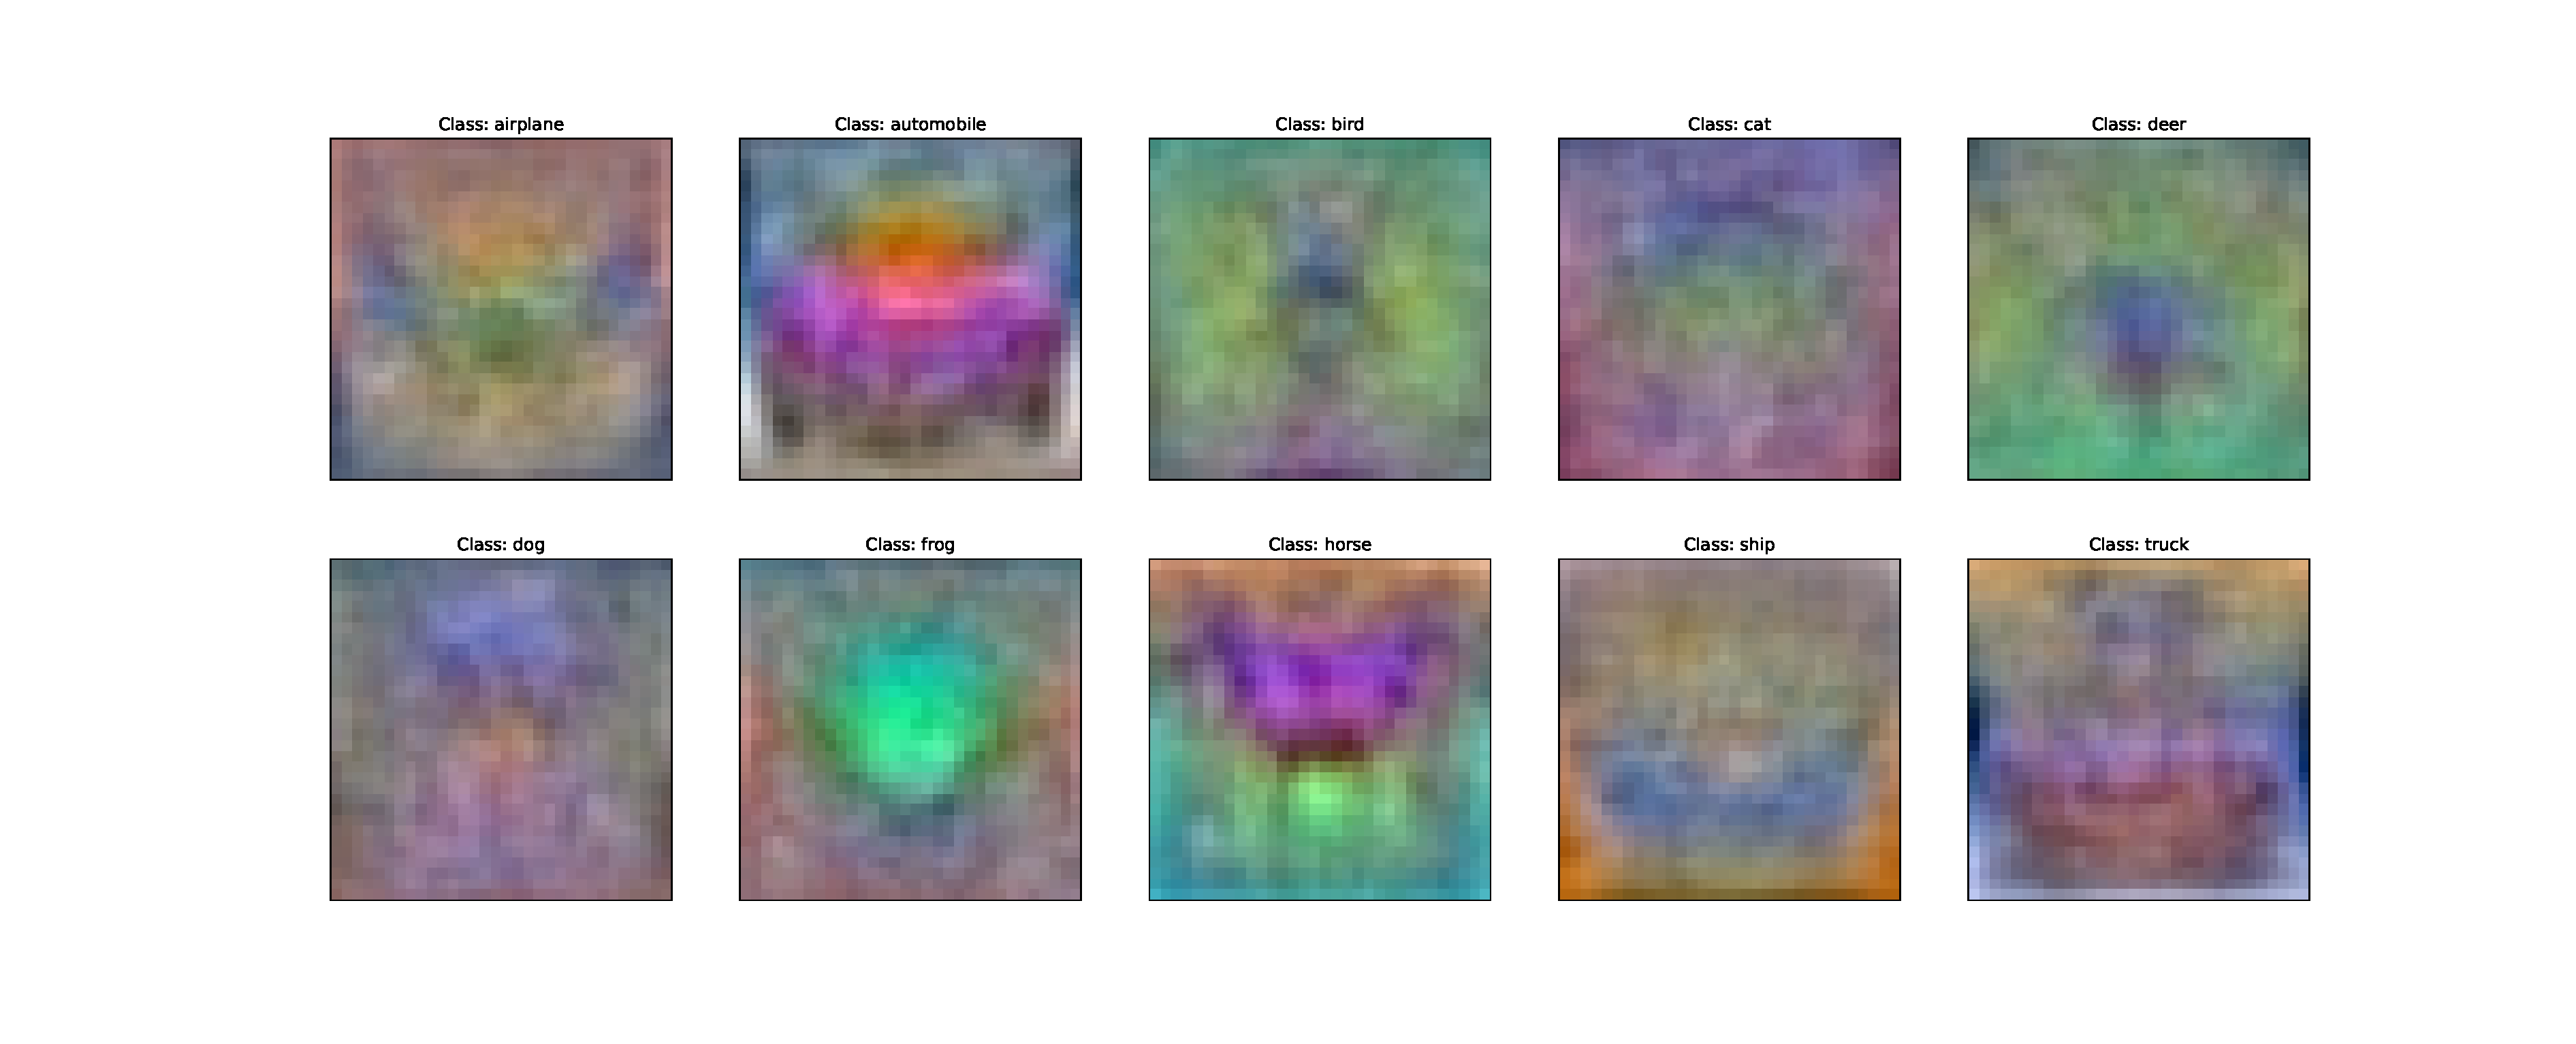
\includegraphics[scale=0.3]{figures/trainedWeightslc}
	\caption{Weights matrix W1 as 10 images}
\end{figure}

\begin{figure}[!h]
	\centering
	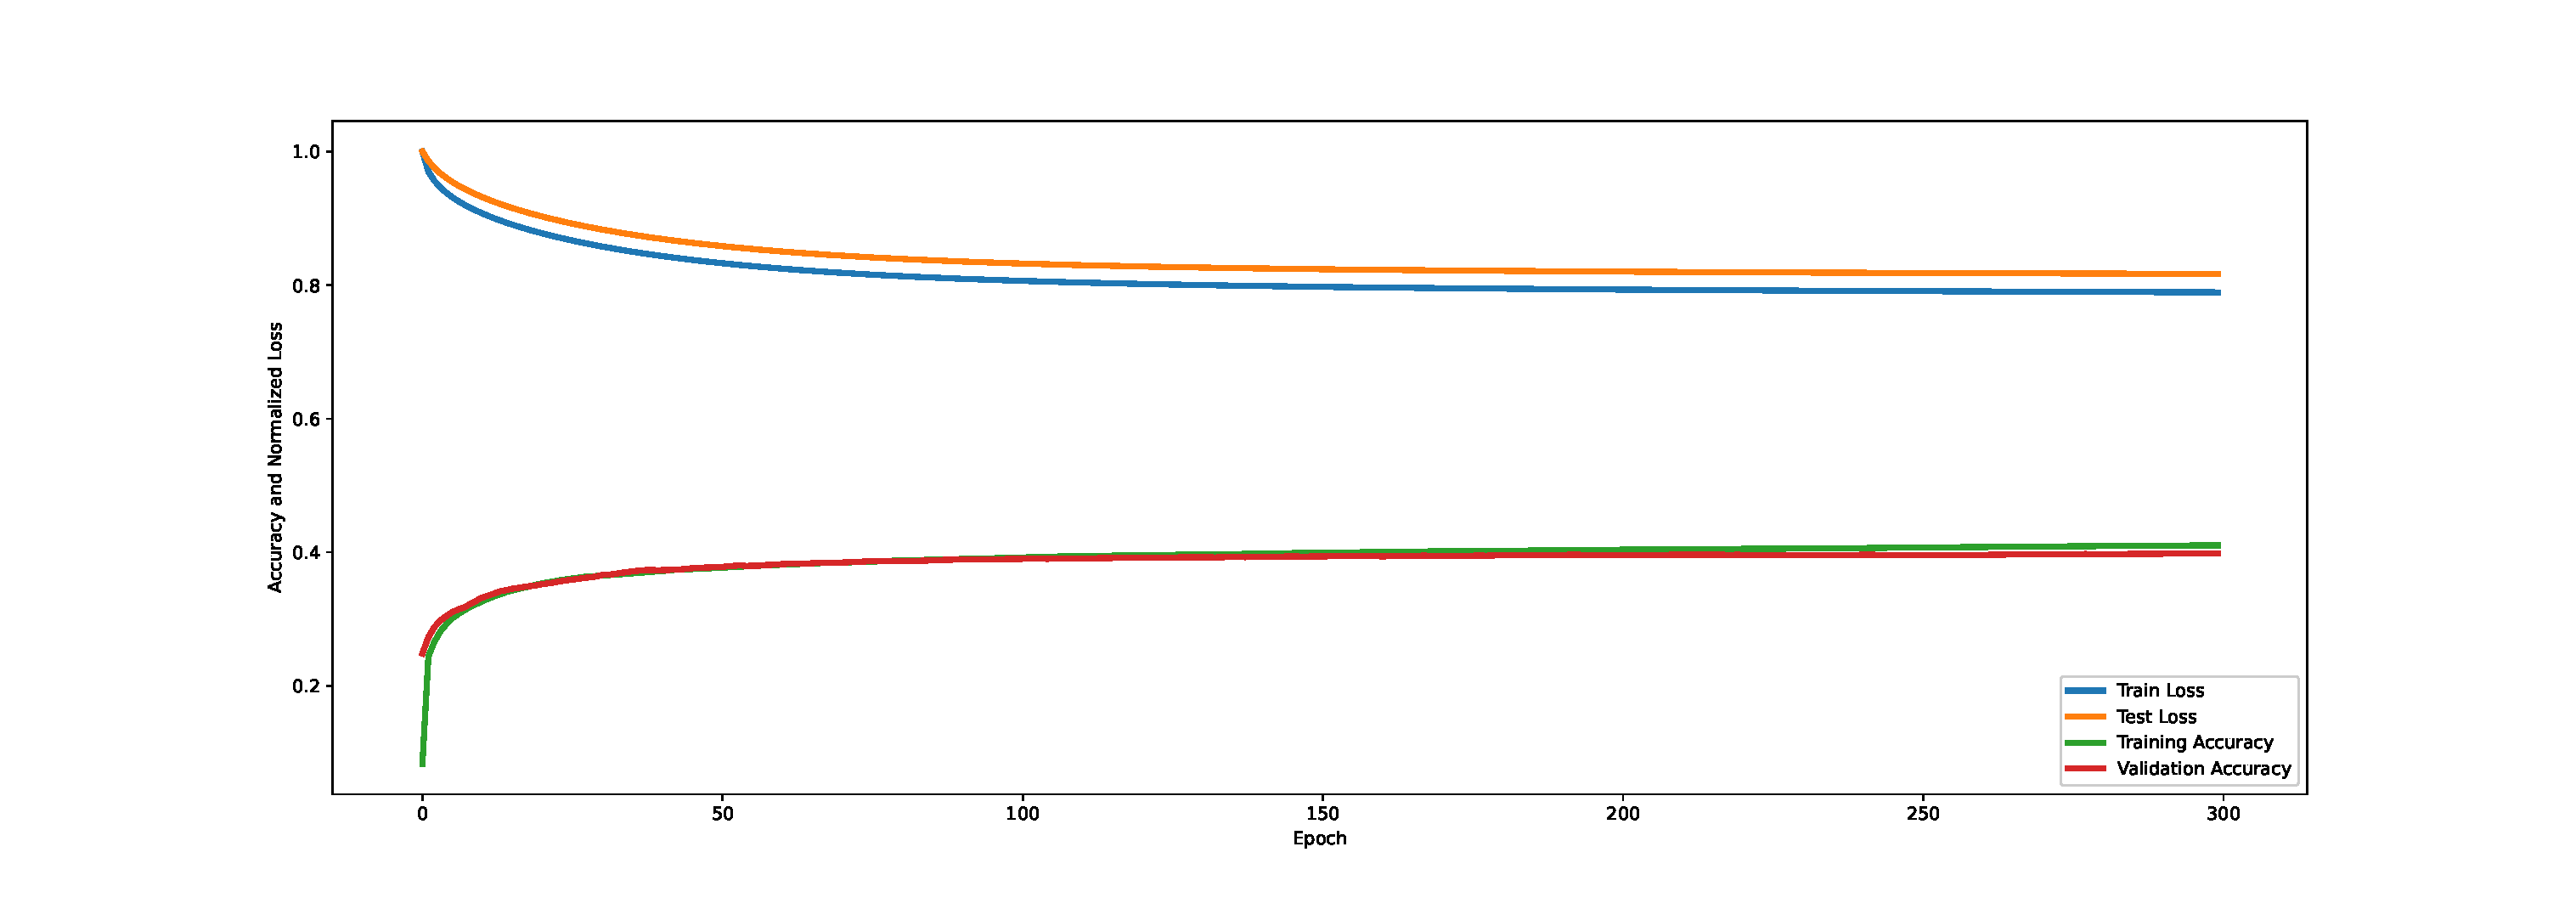
\includegraphics[scale=0.25]{figures/part1plots}
	\caption{Loss, Training Accuracy, Validation Accuracy and Learning Rate of the Linear Classifier with each iteration: for 300 epochs}
\end{figure}

    \begin{tcolorbox}[breakable, size=fbox, boxrule=1pt, pad at break*=1mm,colback=cellbackground, colframe=cellborder]
\prompt{In}{incolor}{5}{\boxspacing}
\begin{Verbatim}[commandchars=\\\{\}]
\PY{n}{H} \PY{o}{=} \PY{l+m+mi}{200} \PY{c+c1}{\PYZsh{} No of hidden nodes}
\PY{n}{std}\PY{o}{=}\PY{l+m+mf}{1e\PYZhy{}5} 
\PY{c+c1}{\PYZsh{} Hidden Layer }
\PY{n}{w1} \PY{o}{=} \PY{n}{std}\PY{o}{*}\PY{n}{np}\PY{o}{.}\PY{n}{random}\PY{o}{.}\PY{n}{randn}\PY{p}{(}\PY{n}{Din}\PY{p}{,} \PY{n}{H}\PY{p}{)} \PY{c+c1}{\PYZsh{} Initializing the weight matrix with random weights}
\PY{n}{b1} \PY{o}{=} \PY{n}{np}\PY{o}{.}\PY{n}{zeros}\PY{p}{(}\PY{n}{H}\PY{p}{)} \PY{c+c1}{\PYZsh{} Initializing the bias vector}
\PY{c+c1}{\PYZsh{} Last Layer}
\PY{n}{w2} \PY{o}{=} \PY{n}{std}\PY{o}{*}\PY{n}{np}\PY{o}{.}\PY{n}{random}\PY{o}{.}\PY{n}{randn}\PY{p}{(}\PY{n}{H}\PY{p}{,} \PY{n}{K}\PY{p}{)} \PY{c+c1}{\PYZsh{} Initializing the weight matrix with random weights}
\PY{n}{b2} \PY{o}{=} \PY{n}{np}\PY{o}{.}\PY{n}{zeros}\PY{p}{(}\PY{n}{K}\PY{p}{)} \PY{c+c1}{\PYZsh{} Initializing the bias vector}
\PY{c+c1}{\PYZsh{} Rearranging train and test samples: (ra=rearranged)}
\PY{n}{x\PYZus{}train\PYZus{}ra} \PY{o}{=} \PY{n}{np}\PY{o}{.}\PY{n}{concatenate}\PY{p}{(}\PY{p}{(}\PY{n}{np}\PY{o}{.}\PY{n}{ones}\PY{p}{(}\PY{p}{(}\PY{n}{x\PYZus{}train}\PY{o}{.}\PY{n}{shape}\PY{p}{[}\PY{l+m+mi}{0}\PY{p}{]}\PY{p}{,}\PY{l+m+mi}{1}\PY{p}{)}\PY{p}{)}\PY{p}{,}\PY{n}{x\PYZus{}train}\PY{p}{)}\PY{p}{,} \PY{n}{axis}\PY{o}{=}\PY{l+m+mi}{1}\PY{p}{)}
\PY{n}{x\PYZus{}test\PYZus{}ra}  \PY{o}{=} \PY{n}{np}\PY{o}{.}\PY{n}{concatenate}\PY{p}{(}\PY{p}{(}\PY{n}{np}\PY{o}{.}\PY{n}{ones}\PY{p}{(}\PY{p}{(}\PY{n}{x\PYZus{}test}\PY{o}{.}\PY{n}{shape}\PY{p}{[}\PY{l+m+mi}{0}\PY{p}{]}\PY{p}{,}\PY{l+m+mi}{1}\PY{p}{)}\PY{p}{)}\PY{p}{,}\PY{n}{x\PYZus{}test}\PY{p}{)}\PY{p}{,} \PY{n}{axis}\PY{o}{=}\PY{l+m+mi}{1}\PY{p}{)}
\PY{c+c1}{\PYZsh{} Rearranging weight matrices and bias vectors into single matrices}
\PY{n}{w1} \PY{o}{=} \PY{n}{np}\PY{o}{.}\PY{n}{concatenate}\PY{p}{(}\PY{p}{(}\PY{n}{b1}\PY{o}{.}\PY{n}{reshape}\PY{p}{(}\PY{l+m+mi}{1}\PY{p}{,}\PY{n}{H}\PY{p}{)}\PY{p}{,} \PY{n}{w1}\PY{p}{)}\PY{p}{,} \PY{n}{axis}\PY{o}{=}\PY{l+m+mi}{0}\PY{p}{)}
\PY{n}{w2} \PY{o}{=} \PY{n}{np}\PY{o}{.}\PY{n}{concatenate}\PY{p}{(}\PY{p}{(}\PY{n}{b2}\PY{o}{.}\PY{n}{reshape}\PY{p}{(}\PY{l+m+mi}{1}\PY{p}{,}\PY{n}{K}\PY{p}{)}\PY{p}{,} \PY{n}{w2}\PY{p}{)}\PY{p}{,} \PY{n}{axis}\PY{o}{=}\PY{l+m+mi}{0}\PY{p}{)}
\end{Verbatim}
\end{tcolorbox}

    \begin{tcolorbox}[breakable, size=fbox, boxrule=1pt, pad at break*=1mm,colback=cellbackground, colframe=cellborder]
\prompt{In}{incolor}{6}{\boxspacing}
\begin{Verbatim}[commandchars=\\\{\}]
\PY{k}{for} \PY{n}{t} \PY{o+ow}{in} \PY{n+nb}{range}\PY{p}{(}\PY{l+m+mi}{1}\PY{p}{,}\PY{n}{iterations}\PY{o}{+}\PY{l+m+mi}{1}\PY{p}{)}\PY{p}{:}
    \PY{c+c1}{\PYZsh{} Forward Propagation}
    \PY{n}{hypo} \PY{o}{=} \PY{n}{sigmoid}\PY{p}{(}\PY{n}{x\PYZus{}train\PYZus{}ra}\PY{o}{.}\PY{n}{dot}\PY{p}{(}\PY{n}{w1}\PY{p}{)}\PY{p}{)} \PY{c+c1}{\PYZsh{} Layer 1 with sigmoid activation}
    \PY{n}{hypothesis} \PY{o}{=} \PY{n}{np}\PY{o}{.}\PY{n}{concatenate}\PY{p}{(}\PY{p}{(}\PY{n}{np}\PY{o}{.}\PY{n}{ones}\PY{p}{(}\PY{p}{(}\PY{n}{hypo}\PY{o}{.}\PY{n}{shape}\PY{p}{[}\PY{l+m+mi}{0}\PY{p}{]}\PY{p}{,}\PY{l+m+mi}{1}\PY{p}{)}\PY{p}{)}\PY{p}{,}\PY{n}{hypo}\PY{p}{)}\PY{p}{,} \PY{n}{axis}\PY{o}{=}\PY{l+m+mi}{1}\PY{p}{)} \PY{c+c1}{\PYZsh{} Rearranging for layer 2}
    \PY{n}{predict} \PY{o}{=} \PY{n}{hypothesis}\PY{o}{.}\PY{n}{dot}\PY{p}{(}\PY{n}{w2}\PY{p}{)} \PY{c+c1}{\PYZsh{} Layer 2     }
    \PY{n}{loss} \PY{o}{=} \PY{p}{(}\PY{l+m+mi}{1}\PY{o}{/}\PY{p}{(}\PY{l+m+mi}{2}\PY{o}{*}\PY{n}{m}\PY{p}{)}\PY{p}{)}\PY{o}{*}\PY{n}{np}\PY{o}{.}\PY{n}{sum}\PY{p}{(}\PY{p}{(} \PY{n}{predict} \PY{o}{\PYZhy{}} \PY{n}{y\PYZus{}train}\PY{p}{)}\PY{o}{*}\PY{o}{*}\PY{l+m+mi}{2}\PY{p}{)}\PYZbs{}
         \PY{o}{+} \PY{p}{(}\PY{l+m+mi}{1}\PY{o}{/}\PY{p}{(}\PY{l+m+mi}{2}\PY{o}{*}\PY{n}{m}\PY{p}{)}\PY{p}{)}\PY{o}{*}\PY{n}{reg}\PY{o}{*}\PY{n}{np}\PY{o}{.}\PY{n}{sum}\PY{p}{(}\PY{n}{w1}\PY{o}{*}\PY{o}{*}\PY{l+m+mi}{2}\PY{p}{)} \PY{o}{+} \PY{p}{(}\PY{l+m+mi}{1}\PY{o}{/}\PY{p}{(}\PY{l+m+mi}{2}\PY{o}{*}\PY{n}{m}\PY{p}{)}\PY{p}{)}\PY{o}{*}\PY{n}{reg}\PY{o}{*}\PY{n}{np}\PY{o}{.}\PY{n}{sum}\PY{p}{(}\PY{n}{w2}\PY{o}{*}\PY{o}{*}\PY{l+m+mi}{2}\PY{p}{)}
    \PY{c+c1}{\PYZsh{} Back Propagation partial dertivatives of Loss function}
    \PY{n}{dpredict} \PY{o}{=}  \PY{p}{(}\PY{l+m+mi}{1}\PY{o}{/}\PY{n}{m}\PY{p}{)}\PY{o}{*}\PY{p}{(}\PY{n}{predict} \PY{o}{\PYZhy{}} \PY{n}{y\PYZus{}train}\PY{p}{)}
    \PY{n}{dw2} \PY{o}{=} \PY{n}{hypothesis}\PY{o}{.}\PY{n}{T}\PY{o}{.}\PY{n}{dot}\PY{p}{(}\PY{n}{dpredict}\PY{p}{)} \PY{o}{+} \PY{p}{(}\PY{l+m+mi}{1}\PY{o}{/}\PY{n}{m}\PY{p}{)}\PY{o}{*}\PY{n}{reg}\PY{o}{*}\PY{n}{w2}
    \PY{n}{dh} \PY{o}{=} \PY{n}{dpredict}\PY{o}{.}\PY{n}{dot}\PY{p}{(}\PY{n}{w2}\PY{p}{[}\PY{l+m+mi}{1}\PY{p}{:}\PY{p}{,}\PY{p}{]}\PY{o}{.}\PY{n}{T}\PY{p}{)} \PY{c+c1}{\PYZsh{} Removing bias vector w2(201x10)\PYZhy{}\PYZhy{}\PYZgt{} 200x10}
    \PY{n}{dhdxw1} \PY{o}{=} \PY{n}{hypo}\PY{o}{*}\PY{p}{(}\PY{l+m+mi}{1} \PY{o}{\PYZhy{}} \PY{n}{hypo}\PY{p}{)} \PY{c+c1}{\PYZsh{}using hypothesis 50000*200 the one before rearranging.}
    \PY{n}{dw1} \PY{o}{=} \PY{n}{x\PYZus{}train\PYZus{}ra}\PY{o}{.}\PY{n}{T}\PY{o}{.}\PY{n}{dot}\PY{p}{(}\PY{n}{dh}\PY{o}{*}\PY{n}{dhdxw1}\PY{p}{)} \PY{o}{+} \PY{p}{(}\PY{l+m+mi}{1}\PY{o}{/}\PY{n}{m}\PY{p}{)}\PY{o}{*}\PY{n}{reg}\PY{o}{*}\PY{n}{w1}    
    \PY{c+c1}{\PYZsh{} Gradient Descent}
    \PY{n}{w1} \PY{o}{=} \PY{n}{w1} \PY{o}{\PYZhy{}} \PY{n}{lr}\PY{o}{*}\PY{n}{dw1}
    \PY{n}{w2} \PY{o}{=} \PY{n}{w2} \PY{o}{\PYZhy{}} \PY{n}{lr}\PY{o}{*}\PY{n}{dw2}
     \PY{c+c1}{\PYZsh{} Decaying learning rate}
    \PY{n}{lr\PYZus{}hitory}\PY{o}{.}\PY{n}{append}\PY{p}{(}\PY{n}{lr}\PY{p}{)}
    \PY{n}{lr} \PY{o}{=} \PY{n}{lr}\PY{o}{*}\PY{n}{lr\PYZus{}decay}
\end{Verbatim}
\end{tcolorbox}

    \begin{tcolorbox}[breakable, size=fbox, boxrule=1pt, pad at break*=1mm,colback=cellbackground, colframe=cellborder]
\prompt{In}{incolor}{7}{\boxspacing}
\begin{Verbatim}[commandchars=\\\{\}]
\PY{n}{batch\PYZus{}size} \PY{o}{=} \PY{l+m+mi}{500} \PY{c+c1}{\PYZsh{} define the batch size}
\PY{n}{seed} \PY{o}{=} \PY{l+m+mi}{0}\PY{p}{;} \PY{n}{rng} \PY{o}{=} \PY{n}{np}\PY{o}{.}\PY{n}{random}\PY{o}{.}\PY{n}{default\PYZus{}rng}\PY{p}{(}\PY{n}{seed}\PY{o}{=}\PY{n}{seed}\PY{p}{)}
\PY{k}{for} \PY{n}{t} \PY{o+ow}{in} \PY{n+nb}{range}\PY{p}{(}\PY{l+m+mi}{1}\PY{p}{,}\PY{n}{iterations}\PY{o}{+}\PY{l+m+mi}{1}\PY{p}{)}\PY{p}{:}
    \PY{n}{indices} \PY{o}{=} \PY{n}{np}\PY{o}{.}\PY{n}{arange}\PY{p}{(}\PY{n}{Ntr}\PY{p}{)} \PY{c+c1}{\PYZsh{}Number of training samples}
    \PY{n}{rng}\PY{o}{.}\PY{n}{shuffle}\PY{p}{(}\PY{n}{indices}\PY{p}{)}
    \PY{n}{x\PYZus{}train\PYZus{}3} \PY{o}{=} \PY{n}{x\PYZus{}train\PYZus{}ra}\PY{p}{[}\PY{n}{indices}\PY{p}{]}
    \PY{n}{y\PYZus{}train\PYZus{}3} \PY{o}{=} \PY{n}{y\PYZus{}train}\PY{p}{[}\PY{n}{indices}\PY{p}{]}
    \PY{n}{batch\PYZus{}loss} \PY{o}{=} \PY{l+m+mi}{0} \PY{c+c1}{\PYZsh{} Loss for each batch}
    \PY{k}{for} \PY{n}{start} \PY{o+ow}{in} \PY{n+nb}{range}\PY{p}{(}\PY{l+m+mi}{0}\PY{p}{,}\PY{n}{Ntr}\PY{p}{,}\PY{n}{batch\PYZus{}size}\PY{p}{)}\PY{p}{:}
        \PY{n}{stop} \PY{o}{=} \PY{n}{start} \PY{o}{+} \PY{n}{batch\PYZus{}size}
        \PY{c+c1}{\PYZsh{} Forward Propagation}
        \PY{n}{hypo} \PY{o}{=} \PY{n}{sigmoid}\PY{p}{(}\PY{n}{x\PYZus{}train\PYZus{}3}\PY{p}{[}\PY{n}{start}\PY{p}{:}\PY{n}{stop}\PY{p}{]}\PY{o}{.}\PY{n}{dot}\PY{p}{(}\PY{n}{w1}\PY{p}{)}\PY{p}{)} \PY{c+c1}{\PYZsh{} Layer 1 with sigmoid activation}
        \PY{n}{hypothesis} \PY{o}{=} \PY{n}{np}\PY{o}{.}\PY{n}{concatenate}\PY{p}{(}\PY{p}{(}\PY{n}{np}\PY{o}{.}\PY{n}{ones}\PY{p}{(}\PY{p}{(}\PY{n}{hypo}\PY{o}{.}\PY{n}{shape}\PY{p}{[}\PY{l+m+mi}{0}\PY{p}{]}\PY{p}{,}\PY{l+m+mi}{1}\PY{p}{)}\PY{p}{)}\PY{p}{,}\PY{n}{hypo}\PY{p}{)}\PY{p}{,} \PY{n}{axis}\PY{o}{=}\PY{l+m+mi}{1}\PY{p}{)} \PY{c+c1}{\PYZsh{} Rearranging for layer 2}
        \PY{n}{predict} \PY{o}{=} \PY{n}{hypothesis}\PY{o}{.}\PY{n}{dot}\PY{p}{(}\PY{n}{w2}\PY{p}{)} \PY{c+c1}{\PYZsh{} Layer 2 }
        \PY{n}{minibatch\PYZus{}loss} \PY{o}{=} \PY{p}{(}\PY{l+m+mi}{1}\PY{o}{/}\PY{p}{(}\PY{l+m+mi}{2}\PY{o}{*}\PY{n}{m}\PY{p}{)}\PY{p}{)}\PY{o}{*}\PY{n}{np}\PY{o}{.}\PY{n}{sum}\PY{p}{(}\PY{p}{(} \PY{n}{predict} \PY{o}{\PYZhy{}} \PY{n}{y\PYZus{}train\PYZus{}3}\PY{p}{[}\PY{n}{start}\PY{p}{:}\PY{n}{stop}\PY{p}{]}\PY{p}{)}\PY{o}{*}\PY{o}{*}\PY{l+m+mi}{2}\PY{p}{)}\PYZbs{}
             \PY{o}{+} \PY{p}{(}\PY{l+m+mi}{1}\PY{o}{/}\PY{p}{(}\PY{l+m+mi}{2}\PY{o}{*}\PY{n}{m}\PY{p}{)}\PY{p}{)}\PY{o}{*}\PY{n}{reg}\PY{o}{*}\PY{n}{np}\PY{o}{.}\PY{n}{sum}\PY{p}{(}\PY{n}{w1}\PY{o}{*}\PY{o}{*}\PY{l+m+mi}{2}\PY{p}{)} \PY{o}{+} \PY{p}{(}\PY{l+m+mi}{1}\PY{o}{/}\PY{p}{(}\PY{l+m+mi}{2}\PY{o}{*}\PY{n}{m}\PY{p}{)}\PY{p}{)}\PY{o}{*}\PY{n}{reg}\PY{o}{*}\PY{n}{np}\PY{o}{.}\PY{n}{sum}\PY{p}{(}\PY{n}{w2}\PY{o}{*}\PY{o}{*}\PY{l+m+mi}{2}\PY{p}{)}
        \PY{n}{batch\PYZus{}loss}\PY{o}{+}\PY{o}{=} \PY{n}{minibatch\PYZus{}loss}
        \PY{c+c1}{\PYZsh{} Back Propagation partial dertivatives of Loss function}
        \PY{n}{dpredict} \PY{o}{=}  \PY{p}{(}\PY{l+m+mi}{1}\PY{o}{/}\PY{n}{m}\PY{p}{)}\PY{o}{*}\PY{p}{(}\PY{n}{predict} \PY{o}{\PYZhy{}} \PY{n}{y\PYZus{}train\PYZus{}3}\PY{p}{[}\PY{n}{start}\PY{p}{:}\PY{n}{stop}\PY{p}{]}\PY{p}{)}
        \PY{n}{dw2} \PY{o}{=} \PY{n}{hypothesis}\PY{o}{.}\PY{n}{T}\PY{o}{.}\PY{n}{dot}\PY{p}{(}\PY{n}{dpredict}\PY{p}{)} \PY{o}{+} \PY{p}{(}\PY{l+m+mi}{1}\PY{o}{/}\PY{n}{m}\PY{p}{)}\PY{o}{*}\PY{n}{reg}\PY{o}{*}\PY{n}{w2}
        \PY{n}{dh} \PY{o}{=} \PY{n}{dpredict}\PY{o}{.}\PY{n}{dot}\PY{p}{(}\PY{n}{w2}\PY{p}{[}\PY{l+m+mi}{1}\PY{p}{:}\PY{p}{,}\PY{p}{]}\PY{o}{.}\PY{n}{T}\PY{p}{)} \PY{c+c1}{\PYZsh{} Removing bias vector w2(201x10)\PYZhy{}\PYZhy{}\PYZgt{} 200x10}
        \PY{n}{dhdxw1} \PY{o}{=} \PY{n}{hypo}\PY{o}{*}\PY{p}{(}\PY{l+m+mi}{1} \PY{o}{\PYZhy{}} \PY{n}{hypo}\PY{p}{)} \PY{c+c1}{\PYZsh{}using hypothesis 50000*200, the one before rearranging.}
        \PY{n}{dw1} \PY{o}{=} \PY{n}{x\PYZus{}train\PYZus{}3}\PY{p}{[}\PY{n}{start}\PY{p}{:}\PY{n}{stop}\PY{p}{]}\PY{o}{.}\PY{n}{T}\PY{o}{.}\PY{n}{dot}\PY{p}{(}\PY{n}{dh}\PY{o}{*}\PY{n}{dhdxw1}\PY{p}{)} \PY{o}{+} \PY{p}{(}\PY{l+m+mi}{1}\PY{o}{/}\PY{n}{m}\PY{p}{)}\PY{o}{*}\PY{n}{reg}\PY{o}{*}\PY{n}{w1}
        \PY{c+c1}{\PYZsh{} Gradient Descent}
        \PY{n}{w1} \PY{o}{=} \PY{n}{w1} \PY{o}{\PYZhy{}} \PY{n}{lr}\PY{o}{*}\PY{n}{dw1}
        \PY{n}{w2} \PY{o}{=} \PY{n}{w2} \PY{o}{\PYZhy{}} \PY{n}{lr}\PY{o}{*}\PY{n}{dw2}    
    \PY{c+c1}{\PYZsh{} Decaying learning rate}
    \PY{n}{lr\PYZus{}hitory}\PY{o}{.}\PY{n}{append}\PY{p}{(}\PY{n}{lr}\PY{p}{)}
    \PY{n}{lr} \PY{o}{=} \PY{n}{lr}\PY{o}{*}\PY{n}{lr\PYZus{}decay}
\end{Verbatim}
\end{tcolorbox}

    \begin{tcolorbox}[breakable, size=fbox, boxrule=1pt, pad at break*=1mm,colback=cellbackground, colframe=cellborder]
\prompt{In}{incolor}{8}{\boxspacing}
\begin{Verbatim}[commandchars=\\\{\}]
\PY{p}{(}\PY{n}{x\PYZus{}train}\PY{p}{,} \PY{n}{y\PYZus{}train}\PY{p}{)}\PY{p}{,} \PY{p}{(}\PY{n}{x\PYZus{}test}\PY{p}{,} \PY{n}{y\PYZus{}test}\PY{p}{)} \PY{o}{=} \PY{n}{datasets}\PY{o}{.}\PY{n}{cifar10}\PY{o}{.}\PY{n}{load\PYZus{}data}\PY{p}{(}\PY{p}{)}
\PY{n}{K} \PY{o}{=} \PY{n+nb}{len}\PY{p}{(}\PY{n}{np}\PY{o}{.}\PY{n}{unique}\PY{p}{(}\PY{n}{y\PYZus{}train}\PY{p}{)}\PY{p}{)} \PY{c+c1}{\PYZsh{} Number of Classes}
\PY{c+c1}{\PYZsh{} Normalize pixel values: Image data preprocessing}
\PY{n}{x\PYZus{}train}\PY{p}{,} \PY{n}{x\PYZus{}test} \PY{o}{=} \PY{n}{x\PYZus{}train} \PY{o}{/} \PY{l+m+mf}{255.0}\PY{p}{,} \PY{n}{x\PYZus{}test} \PY{o}{/} \PY{l+m+mf}{255.0}
\PY{n}{mean\PYZus{}image} \PY{o}{=} \PY{n}{np}\PY{o}{.}\PY{n}{mean}\PY{p}{(}\PY{n}{x\PYZus{}train}\PY{p}{,} \PY{n}{axis}\PY{o}{=}\PY{l+m+mi}{0}\PY{p}{)} \PY{c+c1}{\PYZsh{} axis=0: mean of a column; Mean of each pixel}
\PY{n}{x\PYZus{}train} \PY{o}{=} \PY{n}{x\PYZus{}train} \PY{o}{\PYZhy{}} \PY{n}{mean\PYZus{}image}
\PY{n}{x\PYZus{}test} \PY{o}{=} \PY{n}{x\PYZus{}test} \PY{o}{\PYZhy{}} \PY{n}{mean\PYZus{}image}
\PY{c+c1}{\PYZsh{} Convert class vectors to binary class matrices.}
\PY{n}{y\PYZus{}train} \PY{o}{=} \PY{n}{tf}\PY{o}{.}\PY{n}{keras}\PY{o}{.}\PY{n}{utils}\PY{o}{.}\PY{n}{to\PYZus{}categorical}\PY{p}{(}\PY{n}{y\PYZus{}train}\PY{p}{,} \PY{n}{num\PYZus{}classes}\PY{o}{=}\PY{n}{K}\PY{p}{)}
\PY{n}{y\PYZus{}test} \PY{o}{=} \PY{n}{tf}\PY{o}{.}\PY{n}{keras}\PY{o}{.}\PY{n}{utils}\PY{o}{.}\PY{n}{to\PYZus{}categorical}\PY{p}{(}\PY{n}{y\PYZus{}test}\PY{p}{,} \PY{n}{num\PYZus{}classes}\PY{o}{=}\PY{n}{K}\PY{p}{)}
\PY{c+c1}{\PYZsh{} Declaring the CNN}
\PY{n}{model} \PY{o}{=} \PY{n}{models}\PY{o}{.}\PY{n}{Sequential}\PY{p}{(}\PY{p}{)}
\PY{n}{model}\PY{o}{.}\PY{n}{add}\PY{p}{(}\PY{n}{layers}\PY{o}{.}\PY{n}{Conv2D}\PY{p}{(}\PY{l+m+mi}{32}\PY{p}{,} \PY{p}{(}\PY{l+m+mi}{3}\PY{p}{,} \PY{l+m+mi}{3}\PY{p}{)}\PY{p}{,} \PY{n}{activation}\PY{o}{=}\PY{l+s+s1}{\PYZsq{}}\PY{l+s+s1}{relu}\PY{l+s+s1}{\PYZsq{}}\PY{p}{,} \PY{n}{input\PYZus{}shape}\PY{o}{=}\PY{p}{(}\PY{l+m+mi}{32}\PY{p}{,} \PY{l+m+mi}{32}\PY{p}{,} \PY{l+m+mi}{3}\PY{p}{)}\PY{p}{,} \PY{n}{name}\PY{o}{=}\PY{l+s+s1}{\PYZsq{}}\PY{l+s+s1}{C32}\PY{l+s+s1}{\PYZsq{}}\PY{p}{)}\PY{p}{)}
\PY{n}{model}\PY{o}{.}\PY{n}{add}\PY{p}{(}\PY{n}{layers}\PY{o}{.}\PY{n}{MaxPooling2D}\PY{p}{(}\PY{p}{(}\PY{l+m+mi}{2}\PY{p}{,} \PY{l+m+mi}{2}\PY{p}{)}\PY{p}{)}\PY{p}{)}
\PY{n}{model}\PY{o}{.}\PY{n}{add}\PY{p}{(}\PY{n}{layers}\PY{o}{.}\PY{n}{Conv2D}\PY{p}{(}\PY{l+m+mi}{64}\PY{p}{,} \PY{p}{(}\PY{l+m+mi}{3}\PY{p}{,} \PY{l+m+mi}{3}\PY{p}{)}\PY{p}{,} \PY{n}{activation}\PY{o}{=}\PY{l+s+s1}{\PYZsq{}}\PY{l+s+s1}{relu}\PY{l+s+s1}{\PYZsq{}}\PY{p}{,} \PY{n}{name}\PY{o}{=}\PY{l+s+s1}{\PYZsq{}}\PY{l+s+s1}{C64\PYZus{}1}\PY{l+s+s1}{\PYZsq{}}\PY{p}{)}\PY{p}{)} \PY{c+c1}{\PYZsh{} 64, 3x3 convolutions}
\PY{n}{model}\PY{o}{.}\PY{n}{add}\PY{p}{(}\PY{n}{layers}\PY{o}{.}\PY{n}{MaxPooling2D}\PY{p}{(}\PY{p}{(}\PY{l+m+mi}{2}\PY{p}{,} \PY{l+m+mi}{2}\PY{p}{)}\PY{p}{)}\PY{p}{)}
\PY{n}{model}\PY{o}{.}\PY{n}{add}\PY{p}{(}\PY{n}{layers}\PY{o}{.}\PY{n}{Conv2D}\PY{p}{(}\PY{l+m+mi}{64}\PY{p}{,} \PY{p}{(}\PY{l+m+mi}{3}\PY{p}{,} \PY{l+m+mi}{3}\PY{p}{)}\PY{p}{,} \PY{n}{activation}\PY{o}{=}\PY{l+s+s1}{\PYZsq{}}\PY{l+s+s1}{relu}\PY{l+s+s1}{\PYZsq{}}\PY{p}{,} \PY{n}{name}\PY{o}{=}\PY{l+s+s1}{\PYZsq{}}\PY{l+s+s1}{C64\PYZus{}2}\PY{l+s+s1}{\PYZsq{}}\PY{p}{)}\PY{p}{)} \PY{c+c1}{\PYZsh{} 64, 3x3 convolutions}
\PY{n}{model}\PY{o}{.}\PY{n}{add}\PY{p}{(}\PY{n}{layers}\PY{o}{.}\PY{n}{MaxPooling2D}\PY{p}{(}\PY{p}{(}\PY{l+m+mi}{2}\PY{p}{,} \PY{l+m+mi}{2}\PY{p}{)}\PY{p}{)}\PY{p}{)}
\PY{n}{model}\PY{o}{.}\PY{n}{add}\PY{p}{(}\PY{n}{layers}\PY{o}{.}\PY{n}{Flatten}\PY{p}{(}\PY{p}{)}\PY{p}{)} \PY{c+c1}{\PYZsh{} Make the (None, 2, 2, 64) tensor flat}
\PY{n}{model}\PY{o}{.}\PY{n}{add}\PY{p}{(}\PY{n}{layers}\PY{o}{.}\PY{n}{Dense}\PY{p}{(}\PY{l+m+mi}{64}\PY{p}{,} \PY{n}{activation}\PY{o}{=}\PY{l+s+s1}{\PYZsq{}}\PY{l+s+s1}{relu}\PY{l+s+s1}{\PYZsq{}}\PY{p}{,} \PY{n}{name}\PY{o}{=}\PY{l+s+s1}{\PYZsq{}}\PY{l+s+s1}{F64}\PY{l+s+s1}{\PYZsq{}}\PY{p}{)}\PY{p}{)} \PY{c+c1}{\PYZsh{} Dense Layer 1}
\PY{n}{model}\PY{o}{.}\PY{n}{add}\PY{p}{(}\PY{n}{layers}\PY{o}{.}\PY{n}{Dense}\PY{p}{(}\PY{l+m+mi}{10}\PY{p}{,} \PY{n}{name}\PY{o}{=}\PY{l+s+s1}{\PYZsq{}}\PY{l+s+s1}{F10}\PY{l+s+s1}{\PYZsq{}}\PY{p}{)}\PY{p}{)} \PY{c+c1}{\PYZsh{} Because CIFAR has 10 output classes}
\PY{n}{model}\PY{o}{.}\PY{n}{summary}\PY{p}{(}\PY{p}{)} \PY{c+c1}{\PYZsh{} Complete architecture of the model}
\PY{n}{model}\PY{o}{.}\PY{n}{compile}\PY{p}{(}\PY{n}{optimizer}\PY{o}{=}\PY{n}{tf}\PY{o}{.}\PY{n}{keras}\PY{o}{.}\PY{n}{optimizers}\PY{o}{.}\PY{n}{SGD}\PY{p}{(}\PY{n}{learning\PYZus{}rate}\PY{o}{=}\PY{l+m+mf}{1.4e\PYZhy{}2}\PY{p}{,} \PY{n}{momentum}\PY{o}{=}\PY{l+m+mf}{0.9}\PY{p}{)}\PY{p}{,}
              \PY{n}{loss}\PY{o}{=}\PY{n}{tf}\PY{o}{.}\PY{n}{keras}\PY{o}{.}\PY{n}{losses}\PY{o}{.}\PY{n}{CategoricalCrossentropy}\PY{p}{(}\PY{n}{from\PYZus{}logits}\PY{o}{=}\PY{k+kc}{True}\PY{p}{)}\PY{p}{,}
              \PY{n}{metrics}\PY{o}{=}\PY{p}{[}\PY{l+s+s1}{\PYZsq{}}\PY{l+s+s1}{accuracy}\PY{l+s+s1}{\PYZsq{}}\PY{p}{]}\PY{p}{)}
\PY{n}{history} \PY{o}{=} \PY{n}{model}\PY{o}{.}\PY{n}{fit}\PY{p}{(}\PY{n}{x\PYZus{}train}\PY{p}{,} \PY{n}{y\PYZus{}train}\PY{p}{,}
                    \PY{n}{batch\PYZus{}size}\PY{o}{=}\PY{l+m+mi}{50}\PY{p}{,} \PY{n}{epochs}\PY{o}{=}\PY{l+m+mi}{10}\PY{p}{,} 
                    \PY{n}{validation\PYZus{}data}\PY{o}{=}\PY{p}{(}\PY{n}{x\PYZus{}test}\PY{p}{,} \PY{n}{y\PYZus{}test}\PY{p}{)}\PY{p}{)}
\PY{n}{test\PYZus{}loss}\PY{p}{,} \PY{n}{test\PYZus{}acc} \PY{o}{=} \PY{n}{model}\PY{o}{.}\PY{n}{evaluate}\PY{p}{(}\PY{n}{x\PYZus{}test}\PY{p}{,} \PY{n}{y\PYZus{}test}\PY{p}{,} \PY{n}{verbose}\PY{o}{=}\PY{l+m+mi}{2}\PY{p}{)}
\end{Verbatim}
\end{tcolorbox}
  
\end{document}
